\documentclass[aspectratio=169]{beamer}

% ------------------ XeLaTeX настройки ------------------
\usepackage{fontspec}

\setmainfont{Times New Roman}
\setsansfont{Arial}
\setmonofont{Courier New}

\usepackage{polyglossia}
\setdefaultlanguage{russian}
\uselanguage{russian}
\languagepath{russian}

\deftranslation[to=russian]{Theorem}{Теорема}
\deftranslation[to=russian]{Example}{Пример}
\deftranslation[to=russian]{Proof}{Доказательство}

\newfontfamily\cyrillicfont{Times New Roman}
\newfontfamily\cyrillicfontsf{Arial}
\newfontfamily\cyrillicfonttt{Courier New}

\usepackage{graphicx}
\usepackage{booktabs}
\usepackage{amsmath, amssymb, amsthm}

\usetheme{Madrid}

\setbeamertemplate{caption}[numbered]
\usepackage{caption}
\captionsetup[figure]{
    name=Рисунок,
    labelsep=endash
}
\captionsetup[table]{
    name=Таблица,
    labelsep=endash
}
\setbeamercolor{caption name}{fg=black}
\setbeamercolor{caption}{fg=black}

% ------------------ Теоремы ------------------
\setbeamertemplate{theorems}[numbered]

\newtheorem{proposition}{Утверждение}

% ------------------ Документ ------------------
\title{Автоматизированное распознавание и классификация финансовых транзакций}
\author{Миронов Егор Петрович}
\date{КФУ ИВМиИТ}

\begin{document}

% ======================================================
\begin{frame}
\titlepage
\end{frame}
\transfade 
% ======================================================
\begin{frame}{Оглавление}
\tableofcontents
\end{frame}

% ======================================================
\section{Введение}

\begin{frame}{Введение}
Учебная практика направлена на исследование методов анализа финансовых документов.

\pause

Основная задача:
\begin{itemize}
    \item анализ изображений финансовых документов
    \pause
    \item распознавание транзакций
    \pause
    \item классификация операций
\end{itemize}

\end{frame}

% ======================================================
\section{Проблематика}

\begin{frame}{Актуальность задачи}
Рост цифровых финансовых данных:
\begin{itemize}
    \item кассовый чек
    \item электронный чек
    \item Квитанция об оплате
    \item банковская выписка
    \item скриншот транзакции
    \item фотограия бумажного документа
    \item документы с рукописными элементами
\end{itemize}

\pause

Несмотря на высокий уровень цифровизации, автоматизированная обработка изображений финансовых документов остаётся сложной задачей

\end{frame}

\begin{frame}
На рисунке~\ref{fig:check} продемонстрирован пример типичного документа о транзакции. А в таблице~\ref{tab:docs} перечислены основные такие докуемнты, их источники, а также особенности.
\invisible<1>{
Текст
}
\end{frame}


\begin{frame}{Пример документа о транзакции}
\visible<2->{\begin{figure}
\centering
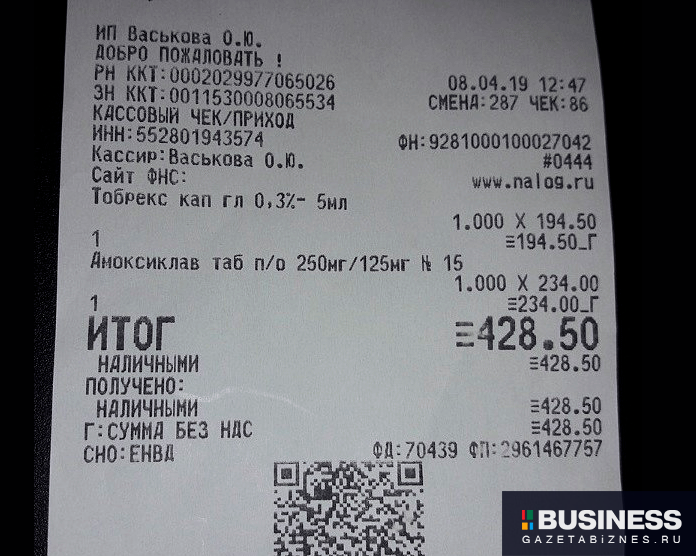
\includegraphics[width=0.45\textwidth]{data/image/check.png}
\caption{Классификация транзакций}
\label{fig:check}
\end{figure}
}
\end{frame}

\begin{frame}{Типы документов}

\begin{table}
\centering
\caption{Типы финансовых документов и их особенности}
\label{tab:docs}

\begin{tabular}{|p{3cm}|p{4cm}|p{5cm}|}
\toprule
Тип документа & Пример источника & Особенности \\
\midrule
Электронный чек & Интернет магазины, маркетплейсы & 
Различные структуры документов, наличие спец. символов \\
\hline
Выписка & 
Интернет-банкинг, PDF-отчеты & 
Сложная сегментация таблиц, переносы строк \\
\hline
Фото фискальных чеков & 
Камера мобильного телефона & 
Геометрические деформации, шумы, потеря читаемости \\
\hline
\end{tabular}
\end{table}


\end{frame}

% ======================================================
\section{OCR и обработка}

\begin{frame}{Оптическое распознавание текста (OCR)}
Функция $f$ описывает процесс преобразования визуального представления
документа в текстовое описание: $f: I \rightarrow T$

\pause

Ключевые этапы стандартного OCR-модуля:
\begin{enumerate}
    \item предобработка входящих данных
    \pause
    \item сегментация изображения
    \pause
    \item распознавание символов
\end{enumerate}

Визуализация такого процесса продемонстрирована на рисунке~\ref{fig:ocr} 


\end{frame}

% ======================================================
\begin{frame}{Пример OCR-процесса}
\begin{figure}
\centering
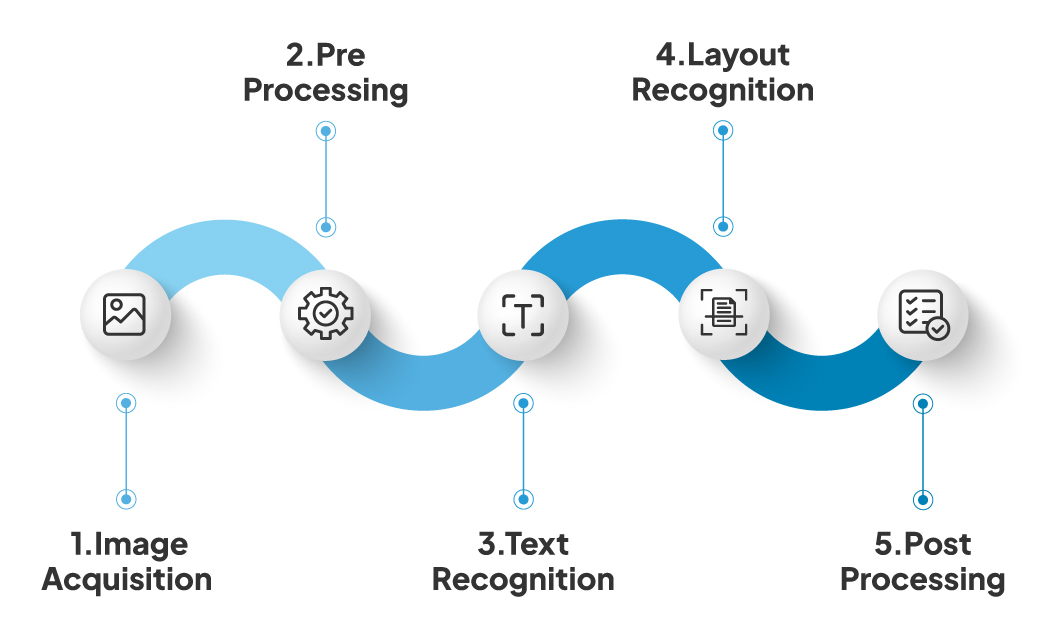
\includegraphics[width=0.7\textwidth]{data/image/ocr.png}
\caption{Процесс OCR обработки}
\label{fig:ocr}
\end{figure}

\end{frame}

% ======================================================
\begin{frame}{Пример OCR-процесса}

Пусть исходное изображение задаётся функцией $I : \Omega \rightarrow \mathbb{R}$, где $\Omega$ --- множество пикселей изображения.
После применения фильтра формируется сглаженное изображение $I_f = G_\sigma * I$.

Двумерное гауссово ядро определяется следующим выражением
$G_\sigma(x,y)=
\frac{1}{2\pi\sigma^2}
\exp\left(
-\frac{x^2+y^2}{2\sigma^2}
\right).$

Применение гауссовой фильтрации позволяет уменьшить влияние
высокочастотного шума и локальных искажений,
сохранив при этом основные структурные элементы текста.

После этапа сглаживания дополнительно может выполняться
бинаризация изображения.
Например, с использованием порогового преобразования 
$
B(x,y)=
\begin{cases}
1, & I_f(x,y) \geq \tau, \\
0, & I_f(x,y) < \tau,
\end{cases}
$.

\end{frame}

% ======================================================
\begin{frame}{Пример OCR-процесса}
Байесовская классификация (обычно Наивный байесовский классификатор) — это вероятностный алгоритм машинного обучения, основанный на теореме Байеса. В контексте финансовых транзакций он используется для автоматической категоризации расходов (например, «Продукты», «Кафе», «Такси»), а также для выявления мошенничества. По обыкновению задается формулой $
P(c \mid \mathbf{x}) =
\frac{P(\mathbf{x} \mid c)\,P(c)}
{\sum_{c' \in \mathcal{C}} P(\mathbf{x} \mid c')\,P(c')}
$
Это очень важная формула в контексте OCR!

\end{frame}

% ======================================================
\section{Извлечение данных}

\begin{frame}{Извлечение структурированной информации}
Формально задачу извлечения структурированной информации
можно представить как отображение: $g : T \rightarrow S$, где: $T=\{t_1,t_2,\dots,t_n\}$ - последовательность токенов, $S=\{(k_i,v_i)\}_{i=1}^{m}$ - множество структурированных пар
ключ-значение.

\pause

Методы:
\begin{itemize}
\item Rule-based методы
\item SVM / Random Forest
\item CNN-based модели
\item RNN / LSTM
\end{itemize}

Сравнение методов представлено в таблице~\ref{tab:methods}

\end{frame}

% ======================================================
\begin{frame}{Сравнение методов}

\begin{table}
\centering
\caption{Сравнение методов обработки}
\label{tab:methods}

\begin{tabular}{|p{2cm}|p{4cm}|p{5cm}|}
\toprule
Метод & Преимущества & Недостатки \\
\midrule
Rule-based методы & Высокая интерпретируемость результатов, простота реализации & Низкая устойчивость к вариативности входных данных \\
\hline
Random Forest & Хорошая работа на небольших выборках & Качество работы существенно зависит от выбранных признаков \\
\hline
RNN/LSTM & Способность учитывать последовательную структуру данных & Медленное обучение и сложность параллелизации вычислений. \\
\hline
\end{tabular}
\end{table}


\end{frame}

% ======================================================
\section{Классификация}

\begin{frame}{Классификация транзакций}
Формально задачу классификации транзакций можно представить как отображение $h : S \rightarrow C$, где $S=\{s_1,s_2,\dots,s_n\}$ --- множество структурированных записей, $C=\{c_1,c_2,\dots,c_k\}$ --- множество категорий транзакций.

\end{frame}

% ======================================================
\begin{frame}{Методы классификации}
    Существующие подходы классификации в рамках рассматриваемой
предметной области \textbf<2>{можно разделить на несколько групп}: 
\begin{itemize}
\item правило-ориентированные методы,
\pause
\item методы машинного обучения,
\pause
\item глубокое обучение и мультимодальные подходы,
\pause
\item смешанные подходы
\end{itemize}
\pause
Причем в большинстве случаев современные модели классификации определяют категорию транзакции как наиболее вероятный класс:
$\hat{c}=
\arg\max_c P(c|s)
$, где $P(c|s)$ представляет вероятность принадлежности
транзакции $s$ классу $c$.

\end{frame}

% ======================================================
\begin{frame}{Embedding-представленияы}

Рассмотрим схему обработки транзакции трансформерной моделью.

\pause
После формирования embedding-представлений последовательность подается в трансформерную модель, 
где механизм self-attention вычисляет зависимости между всеми токенами входной последовательности. $P(y=k \mid \mathbf{x}) =
\frac{\exp(\mathbf{w}_k^\top \mathbf{x})}
{\sum_{j=1}^{K} \exp(\mathbf{w}_j^\top \mathbf{x})}$. Это позволяет модели учитывать глобальный контекст описания транзакции и эффективно выявлять семантические связи между словами.

\end{frame}

% ======================================================
\begin{frame}{Пространства признаков}
Рассмотрим вклад отдельного признака $x_i$ в предсказание модели.
Формально чувствительность выхода можно выразить через градиент:
$
S_i = \frac{\partial f(x)}{\partial x_i}.
$
\pause
В глубокой модели этот градиент раскрывается по правилу цепочки:
$
\frac{\partial f}{\partial x}
=
\prod_{l=1}^{L}
\frac{\partial h_l}{\partial h_{l-1}}
=
\prod_{l=1}^{L}
J_l,
$
\pause
При увеличении $L$ произведение якобианов становится
либо сильно сглаженным, либо нестабильным,
что затрудняет интерпретацию влияния отдельных признаков.

\end{frame}

% ======================================================
\begin{frame}{Двухколоночный слайд (ТЗ требование)}

\begin{columns}

\column{0.5\textwidth}
Полученное контекстное представление используется на этапе классификации для определения категории транзакции, 
например: покупки, переводы, коммунальные платежи или подписки. Схема процесса на рисунке~\ref{fig:pl}

\pause

\column{0.5\textwidth}
\begin{figure}
\centering

\includegraphics[width=0.7\textwidth]{data/image/pipeline.png}
\caption{Классификация транзакций}
\label{fig:pl}
\end{figure}

\end{columns}

\end{frame}

% ======================================================
\section{Теоретическая часть}

\begin{frame}{Теорема и доказательство}

\begin{theorem}
Любая транзакция может быть представлена как вектор признаков в пространстве $\mathbb{R}^n$.
\end{theorem}

\pause

\begin{proof}
Каждый документ содержит конечное число параметров: сумма, дата, тип.
Следовательно, отображение в $\mathbb{R}^n$ существует.
\end{proof}

\end{frame}

% ======================================================
\begin{frame}{Утверждение и пример}

\begin{proposition}
Точность классификации увеличивается при использовании контекста документа.
\end{proposition}

\pause

\begin{example}
Цифровой чек магазина с одинаковой суммой может быть классифицирован как:
\begin{itemize}
\item трата в категории "Еда"
\item трата в категории "Продукты"
\item тараты в категории "Доставка"
\end{itemize}
Контекст того, что чек был сформирован в приложении доставки увеличивает точность верной классификации.
\end{example}

\end{frame}

% ======================================================
\section{Дополнительно}

\begin{frame}{Анимации (ТЗ требование)}

\begin{itemize}
\item<1-> OCR системы
\item<2-> NLP обработка
\item<3-> Классификация
\end{itemize}

\pause

\only<3>{Финальный этап анализа}

\uncover<2->{Промежуточная обработка данных}

\alt<1>{Начало процесса}{Продолжение обработки}

\onslide<2->{
Текст появится со 2 overlay
}

\end{frame}

% ======================================================
\begin{frame}{Дополнительные формулы}

\[
\mathcal{L} = -\log P(y \mid x) 
= -\log \frac{e^{w_y^\top x}}{\sum_k e^{w_k^\top x}} 
= - w_y^\top x + \log \sum_k e^{w_k^\top x}
\]

\[
Q(\theta \mid \theta^{(t)}) =
\mathbb{E}_{Z \sim P(Z \mid X, \theta^{(t)})}
[\log P(X, Z \mid \theta)] 
\theta^{(t+1)} = \arg\max_{\theta} Q(\theta \mid \theta^{(t)})
\]

\[
\hat{\mathbf{y}} = \arg\max_{\mathbf{y}} P(\mathbf{y} \mid \mathbf{x}) 
= \arg\max_{\mathbf{y}} \sum_t \log P(y_t \mid y_{t-1}, x)
\]

\end{frame}

% ======================================================
\section{Заключение}

\begin{frame}{Заключение}

\begin{itemize}
\item Исследованы OCR методы
\item Проанализированы ML подходы
\item Выявлена проблема универсальности
\end{itemize}

\pause

Итог:
\[
\text{Необходим модульный подход}
\]

\end{frame}

% ======================================================
\begin{frame}{Список литературы}

\begin{thebibliography}{3}

\bibitem{1} Современное состояние отечественных цифровых экосистем как
элемента потребительского рынка онлайн торговли / М. В. Шендо, Е. В. Сви-
ридова, М. В. Липаев, А. П. Володин.

\bibitem{2} Роль технологий искусственного интеллекта в цифровой транс-
формации экономики / Е. А. Яковлева, А. Н. Виноградов, Л. В. Александро-
ва, А. П. Филимонов.

\bibitem{3} Пантелеева А. И. Применение компьютерного зрения для анализа
графической информации в экономике.

\end{thebibliography}

\end{frame}

% ======================================================
\end{document}